\pagestyle{fancy}
\vspace*{40 pt}

\subsection{Tela progresso do ajuste}

Esta tela fornece uma representação visual do progresso do ajuste, enquanto o ajuste está sendo realizado os circulos são preenchidos com a cor amarela, quando o ajuste 
é concluído os circulos são preenchidos com a cor verde e quando algum erro ocorre o círculo é preenchido pela cor alaranjada. Também existe uma barra que aumenta de tamanho
conforme o ajuste é concluído.
Esta tela é exibida quando o operador clica no botão "Ajustar" na tela \nameref{sec:telaCarregandoPedido}, ver: \ref{sec:telaCarregandoPedidoDetalhesReceita} - 
\nameref{sec:telaCarregandoPedidoDetalhesReceita}. Clicando em "Cancelar" o ajuste é interrompido e a tela anterior inicial é exibida. Ao clicar em "Voltar" a tela inicial é 
exibida porém sem cancelar o processo de ajuste em andamento. Para voltar a visualizar esta tela basta clicar em pedidos, porém quando o processo é concluído o botão "Cancelar" 
muda para o estado "Finalizar" impedindo o aparecimento do status do ajuste quando é selecionada a tela de pedidos.

\vspace*{\fill}
\begin{figure}[h]
    \centering
    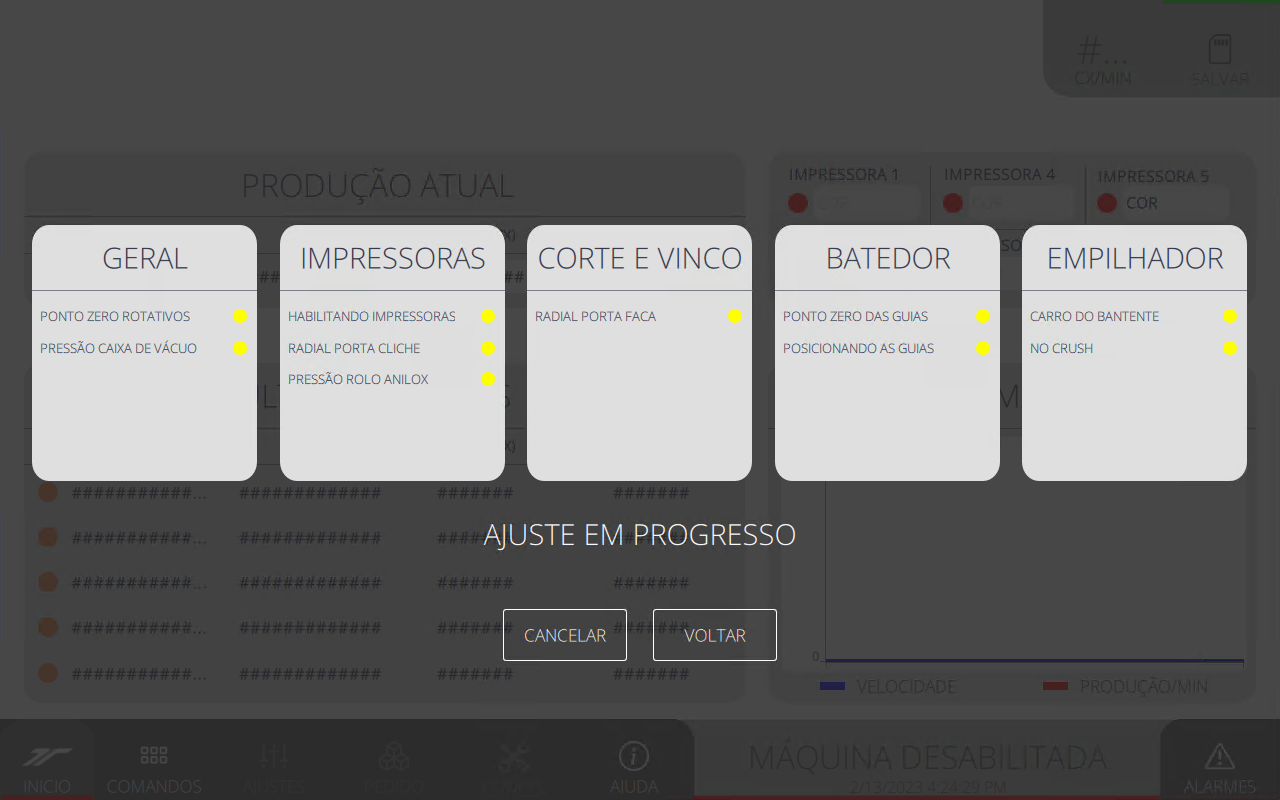
\includegraphics[width=480 px,height=300 px]{src/imagesICV/15-setupProgress/1.png}
\end{figure}
\vspace*{\fill}